\documentclass[twocolumn,11pt,a4paper]{article}

% ====== PAQUETES ======
\usepackage[utf8]{inputenc}
\usepackage[T1]{fontenc}
\usepackage[spanish]{babel}
\usepackage{geometry}
\usepackage{setspace}
\usepackage{graphicx}
\usepackage{fancyhdr}
\usepackage{titlesec}
\usepackage{float}
\usepackage{hyperref}
\usepackage{url}
\usepackage{caption}
\usepackage{natbib}
\usepackage{ragged2e}
\bibliographystyle{apalike}
\usepackage{enumitem}
\setlist[itemize]{itemsep=0pt, topsep=4pt, parsep=0pt, partopsep=0pt}
\usepackage{helvet}
\renewcommand{\familydefault}{\sfdefault}
\justifying

% ====== CONFIGURACIÓN APA ======
\geometry{top=2.5cm, bottom=2.5cm, left=3cm, right=3cm}
\setlength{\columnsep}{0.75cm}
\setlength{\parindent}{0.5cm}
\setstretch{1.15}
\setlength{\headheight}{14pt}

\hypersetup{
    colorlinks=true,
    linkcolor=black,
    citecolor=black,
    urlcolor=blue
}

\pagestyle{fancy}
\fancyhf{}
\fancyhead[R]{\thepage}

% ====== FORMATO DE SECCIONES ======
\titleformat{\section}{\bfseries\normalsize}{\thesection.}{0.5em}{\uppercase}
\titleformat{\subsection}{\normalsize\bfseries}{\thesubsection.}{0.5em}{}

% ====== PORTADA ======
\title{\textbf{\LARGE NodeAlert IoT: Sistema de Monitoreo Ambiental para la Detección Temprana de Condiciones Peligrosas}\\[1cm]
\large Un proyecto académico presentado en la Universidad Nacional de Rafaela\\[3cm]}

\author{
\Large Eloy Kirov, Francisco Alemandi, Palavecino Sebastian\\[0.5cm]
\textit{Universidad Nacional de Rafaela (UNRaf)}\\
\textit{Ingeniería en Computación}\\[0.5cm]
Docentes: Ing. Milton Pozzo, Ing. Matias Wanzenried\\[1cm]
\textbf{26 de noviembre de 2025}
}

\date{}

% ====== DOCUMENTO ======
\begin{document}

\maketitle
\thispagestyle{empty}
\newpage

\twocolumn[
\vspace{-0.5cm}
\begin{center}
\rule{8cm}{0.4pt}
\end{center}
\vspace{0.3cm}
]

% ====== CONTENIDO =====
%===========================================================================0
%==============================================================================
%===========================================================================0%===========================================================================0
%==============================================================================
%===========================================================================0%===========================================================================0
%==============================================================================
%===========================================================================0%===========================================================================0
%==============================================================================
%===========================================================================0%===========================================================================0
%==============================================================================
%===========================================================================0%===========================================================================0
% ====== CONTENIDO ======
\section{Resumen}
El presente trabajo expone la evolución del sistema \textit{FireSafe} hacia una arquitectura de Internet de las Cosas (IoT) distribuida, diseñada para el monitoreo ambiental crítico y la detección temprana de riesgos. A diferencia de su predecesor, esta versión implementa una topología de red en la que múltiples nodos periféricos basados en el microcontrolador ESP32 realizan el procesamiento en el borde (\textit{Edge Computing}), gestionando la concurrencia de tareas mediante el sistema operativo de tiempo real FreeRTOS \citep{valvano2014volume1}. 

La infraestructura se apoya en un protocolo de mensajería asíncrona MQTT bajo un modelo de publicación/suscripción, garantizando una comunicación eficiente y escalable entre los nodos y el servidor central en una Raspberry Pi. El sistema integra un \textit{backend} desarrollado en Django para la persistencia de datos y un \textit{dashboard} interactivo en React que permite la visualización en tiempo real y la gestión de alertas. Los resultados demuestran que el análisis de circuitos propuesto por \citet{boylestad2009} y la implementación de interfaces de tiempo real \citep{valvano2014volume2} permiten una respuesta inmediata ante fluctuaciones térmicas o presencia de gases combustibles, validando la viabilidad de soluciones industriales de bajo costo.

\textbf{Palabras clave:} IoT distribuido, MQTT, FreeRTOS, monitoreo ambiental, sistemas de tiempo real.
\vspace{0.5cm}
\section{Abstract}
This paper presents the evolution of the \textit{FireSafe} system towards a distributed Internet of Things (IoT) architecture, designed for critical environmental monitoring and early hazard detection. Unlike its predecessor, this version implements a network topology where multiple ESP32-based peripheral nodes perform edge computing, managing task concurrency through the FreeRTOS real-time operating system \citep{valvano2014volume1}. 

The infrastructure is supported by the MQTT asynchronous messaging protocol under a publish/subscribe model, ensuring efficient and scalable communication between nodes and the central server on a Raspberry Pi. The system integrates a Django-developed backend for data persistence and a React-based interactive dashboard for real-time visualization and automatic alert management. The results demonstrate that the circuit analysis proposed by \citet{boylestad2009} and the implementation of real-time interfacing \citep{valvano2014volume2} allow for an immediate response to thermal fluctuations or the presence of combustible gases, validating the feasibility of low-cost industrial solutions.

\textbf{Keywords:} Distributed IoT, MQTT, FreeRTOS, environmental monitoring, real-time systems.

\section{Introducción}
La seguridad en entornos habitacionales e industriales representa uno de los pilares fundamentales del bienestar humano y la preservación de activos materiales. En particular, la prevención y detección temprana de incendios y fugas de gases peligrosos constituye un desafío técnico crítico, dado que el tiempo de respuesta es inversamente proporcional a la magnitud de los daños resultantes. Históricamente, la ingeniería ha abordado esta problemática mediante dispositivos aislados; sin embargo, la complejidad de las infraestructuras modernas demanda soluciones integrales que operen de manera coordinada.

En la última década, la arquitectura de la \textit{Internet de las Cosas} (IoT) ha transformado radicalmente este panorama. El despliegue de redes de sensores inalámbricos (\textit{Wireless Sensor Networks}) permite no solo capturar variables físicas como temperatura, humedad y concentración de gases combustibles, sino también procesar dicha información de forma distribuida. Según \citet{valvano2014volume1}, un sistema embebido moderno no debe limitarse a la captura de datos, sino que debe integrar capacidades de comunicación y procesamiento en tiempo real para tomar decisiones autónomas y eficientes.

Bajo esta premisa, el proyecto \textit{NodeAlert IoT } evoluciona de un prototipo de monitoreo único a un ecosistema distribuido basado en la arquitectura \textit{Edge Computing}. Esta transición permite que el procesamiento de señales críticas basado en los principios fundamentales de circuitos eléctricos \citep{alexander2006}  se realice en la periferia de la red (nodos ESP32), reduciendo la latencia y la dependencia de un servidor central. 

La implementación de este sistema se fundamenta en la integración de protocolos de comunicación robustos como MQTT y el uso de sistemas operativos de tiempo real (RTOS) para la gestión de tareas concurrentes . A lo largo de este documento, se detallará cómo esta arquitectura no solo mejora la confiabilidad de la detección, sino que también ofrece una escalabilidad industrial, permitiendo la supervisión remota mediante interfaces web, consolidando una solución accesible y de alto rendimiento para la gestión de emergencias ambientales.
\section{Estado del Arte}
La evolución de los sistemas de monitoreo ambiental ha transitado desde dispositivos analógicos aislados hacia ecosistemas complejos de \textit{Wireless Sensor Networks} (WSN) integrados en arquitecturas de Smart Buildings e Industria 4.0. El estado actual de la técnica se define por la capacidad de procesar datos en la periferia (\textit{Edge Computing}) y la interoperabilidad mediante protocolos ligeros.

\subsection{Sistemas SCADA y Monitoreo Industrial}
Históricamente, el monitoreo industrial ha dependido de sistemas de Control Supervisorio y Adquisición de Datos (SCADA). Sin embargo, los sistemas SCADA tradicionales suelen ser rígidos y centralizados. La tendencia moderna, impulsada por el IoT Industrial (IIoT), propone una transición hacia sistemas distribuidos donde cada nodo posee capacidad de cómputo independiente. Según \citet{valvano2014volume2}, el diseño de interfaces de tiempo real es el núcleo que permite a estos sistemas responder a eventos asíncronos con determinismo, superando la latencia de los sistemas de sondeo (\textit{polling}) convencionales.

\subsection{Redes de Sensores Inalámbricos (WSN) y MQTT}
El despliegue de redes \textit{NodeAlert IoT } se fundamenta en el concepto de WSN, donde la topología de red permite una cobertura extensa sin dependencia de cableado estructurado. El estándar de comunicación \textit{de facto} para estas redes es el protocolo MQTT (\textit{Message Queuing Telemetry Transport}). La literatura técnica destaca que la eficiencia de MQTT radica en su modelo de publicación/suscripción, ideal para dispositivos con recursos limitados de memoria y energía \citep{mazidi2014}. Esto permite la creación de sistemas de mensajería asíncrona que pueden escalar desde un entorno doméstico hasta una infraestructura de \textit{Smart Building}.

\subsection{Edge Computing y Sistemas Distribuidos Embebidos}
Una limitación crítica en el estado del arte previo era la dependencia de la nube para la toma de decisiones. El \textit{Edge Computing} resuelve esto procesando la lógica de control localmente en el nodo central o \textit{gateway}. \citet{valvano2014volume1} sostiene que la robustez de un sistema distribuido embebido reside en su capacidad de mantener la operatividad incluso ante la pérdida de conectividad externa. La integración de sistemas operativos de tiempo real (RTOS) en nodos periféricos como el ESP32 garantiza que la captura de señales críticas, como las descritas en la teoría de dispositivos electrónicos de \citet{boylestad2009}, no se vea interrumpida por las tareas de comunicación de red.

En este contexto, \textit{NodeAlert IoT} no solo actúa como un detector, sino como un sistema embebido distribuido que integra supervisión remota, alertas automáticas y lógica de control local, cerrando la brecha entre los prototipos académicos y las soluciones industriales escalables.
\section{Arquitectura General del Sistema}
La arquitectura de \textit{NodeAlert IoT} se fundamenta en un modelo jerárquico y distribuido que separa las tareas de adquisición, gestión de red y servicios de aplicación. Esta estructura, alineada con las arquitecturas modernas de \textit{Internet of Things} (IoT), garantiza que el sistema sea escalable y presente una alta tolerancia a fallos en entornos críticos.

\subsection{Descripción del Ecosistema}
El ecosistema se organiza en tres capas funcionales, permitiendo que cada componente opere con el determinismo requerido para sistemas de tiempo real \citep{valvano2014volume2}:

\begin{enumerate}[label=\alph*)]
    \item \textbf{Capa de Percepción (Nodos ESP32):} Conformada por múltiples nodos basados en el microcontrolador ESP32. Cada nodo actúa como una unidad de procesamiento en el borde (\textit{Edge Node}), encargada de la lectura de sensores ambientales (DHT22, MQ-9, KY-026), la ejecución de lógica de control local inmediata y la activación de un buzzer de alarma ante condiciones peligrosas. Los nodos se conectan directamente al broker MQTT por WiFi sin necesidad de un gateway intermedio.
    \item \textbf{Capa de Servidor (Raspberry Pi):} Una Raspberry Pi ejecuta Docker Compose con cuatro servicios: el broker MQTT Mosquitto para la mensajería asíncrona, el backend Django con MySQL para la persistencia y API REST, el frontend React servido por Nginx, y Nginx como proxy reverso.
    \item \textbf{Capa de Aplicación:} El punto de interacción con el usuario final, compuesto por un \textit{dashboard} web desarrollado en React con Material UI para monitoreo en tiempo real, visualización de gráficos históricos y envío de comandos a los nodos.
\end{enumerate}
\begin{figure}[H]
    \centering
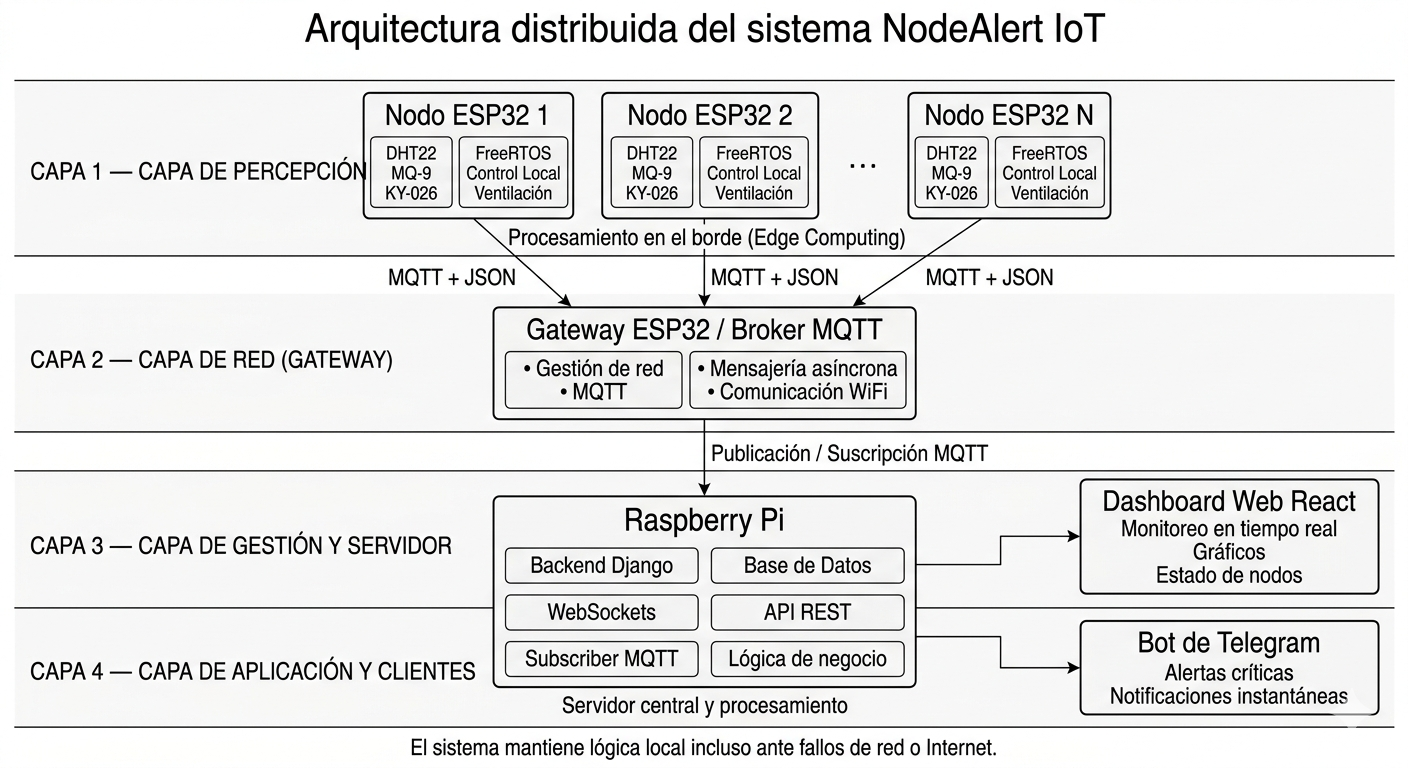
\includegraphics[width=1.1\linewidth]{aqrdistru.png}
    \caption{Arquitectura distribuida del sistema NodeAlert IoT: Interacción entre Nodos ESP32, Raspberry Pi y Cliente Web.}
     \label{fig:arquitectura_general}
 \end{figure}

\subsection{Flujo de Datos y Comunicación}
El flujo de información comienza con la digitalización de señales analógicas en los nodos periféricos, siguiendo los principios de análisis de circuitos de \citet{alexander2006}. Los datos se empaquetan en formato JSON y se publican en tópicos específicos de MQTT. 

La separación de estas capas asegura que, incluso si el servidor central o la conexión a Internet fallan, los nodos individuales mantengan la capacidad de ejecutar acciones preventivas locales, cumpliendo con los requisitos de seguridad descritos por \citet{valvano2014volume1} para sistemas embebidos de misión crítica.

% FOTO REAL: aqrdistru.png
\section{Diseño de Hardware}

El diseño del hardware de \textit{NodeAlert IoT} adopta un enfoque de diseño por capas, lo que permite una clara separación de funciones y facilita el mantenimiento y la escalabilidad.

\subsection{Nodos IoT Periféricos (Capa de Adquisición)}
Los nodos periféricos están centrados en el microcontrolador ESP32 debido a su capacidad de procesamiento de doble núcleo y conectividad Wi-Fi integrada. Estos nodos son los encargados de interactuar directamente con el entorno físico.

\begin{itemize}
    \item \textbf{Sensores:} Se utilizan sensores de respuesta rápida para variables críticas. Según \citet{boylestad2009}, el tiempo de recuperación y la sensibilidad de los dispositivos semiconductores son vitales para la precisión. Se integran:
    \begin{itemize}
        \item \textbf{DHT22:} Para humedad y temperatura, con comunicación digital.
        \item \textbf{MQ-9:} Sensor electroquímico para detección de monóxido de carbono y gases inflamables.
        \item \textbf{KY-026:} Sensor infrarrojo para detección de espectro de llama.
    \end{itemize}
    \item \textbf{Actuador (Buzzer):} Cada nodo cuenta con un buzzer activo conectado al GPIO2 a través de un transistor 2N2222 con resistencia de base de 1k$\Omega$, necesario porque el buzzer consume entre 50 y 100mA, superando la corriente máxima de 40mA del GPIO. El buzzer reproduce patrones diferenciados seg\'un la severidad de la alerta (WARNING, CRITICAL, EMERGENCY).
\end{itemize}

\subsection{Servidor (Raspberry Pi)}
La infraestructura central reside en una \textbf{Raspberry Pi}, que ejecuta los siguientes servicios mediante Docker Compose:
\begin{itemize}
    \item \textbf{Broker Mosquitto:} Servicio MQTT que centraliza la mensajer\'ia as\'incrona entre los nodos ESP32 y el backend Django.
    \item \textbf{Django + MySQL:} Backend que ejecuta un subscriptor MQTT en segundo plano para persister las lecturas de sensores, y expone una API REST para consultas hist\'oricas y env\'io de comandos a los nodos.
    \item \textbf{Frontend React:} Aplicaci\'on web servida por Nginx que consume la API REST para visualizar datos en tiempo real.
    \item \textbf{Nginx:} Proxy reverso que sirve el frontend y enruta las peticiones API a Django.
\end{itemize}
 \begin{figure}[H]
     \centering
     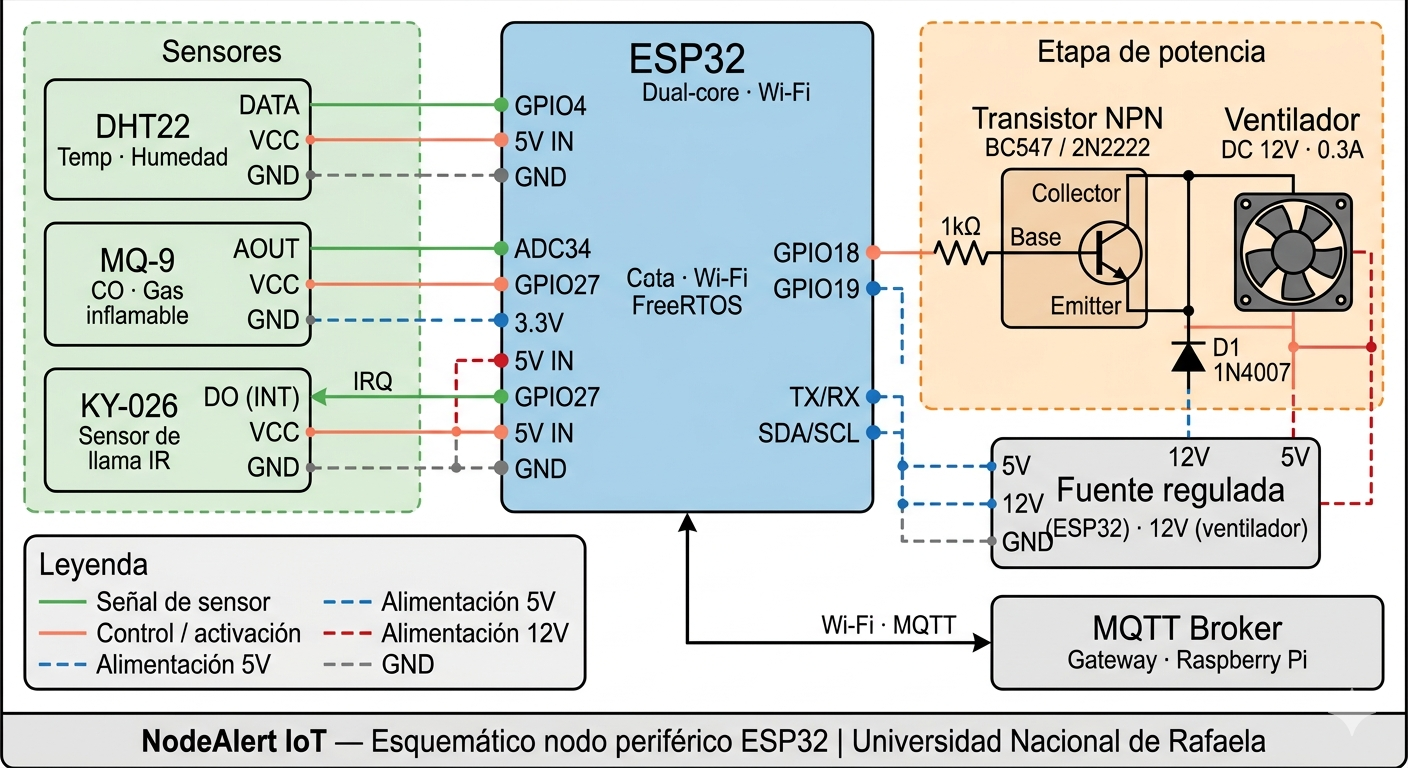
\includegraphics[width=0.9\linewidth]{esdd.png}
     \caption{Esquemático detallado del nodo periférico: Conexiones de sensores y etapa de potencia para el buzzer.}
    \label{fig:esquematico_hard}
 \end{figure}

% FOTO REAL: esdd.png
\section{Diseño de Software y Firmware}

El componente de software de \textit{NodeAlert IoT} se divide en tres dominios críticos: el firmware de los nodos periféricos, la lógica del servidor central y la interfaz de usuario, se ha adoptado un enfoque modular que facilita la depuración y la actualización del sistema.

\subsection{Firmware y Gestión de Tareas (FreeRTOS)}
A diferencia de los sistemas tradicionales basados en un único bucle de ejecución, los nodos ESP32 operan bajo el núcleo de \textbf{FreeRTOS}. Esto permite una ejecución concurrente de tareas con diferentes niveles de prioridad, un concepto fundamental para sistemas de tiempo real \citep{valvano2014volume2}.
\begin{itemize}
    \item \textbf{Tarea de Adquisición:} Encargada del muestreo de sensores en intervalos precisos.
    \item \textbf{Tarea de Comunicación:} Gestiona la conexión Wi-Fi y la publicación de mensajes MQTT sin bloquear la lectura de los sensores.
    \item \textbf{Manejo de Interrupciones:} Se utilizan interrupciones externas para sensores críticos como el de llama (KY-026), asegurando una respuesta inmediata que no dependa del tiempo de ciclo del software.
\end{itemize}

\subsection{Backend y Persistencia de Datos (Django)}
El servidor central, alojado en la Raspberry Pi, utiliza el \textit{framework} Django Esta elección permite manejar la lógica de negocio y la persistencia en base de datos mediante un ORM (\textit{Object-Relational Mapping}) robusto. 
\begin{itemize}
    \item \textbf{MQTT Subscriber:} Un servicio en segundo plano escucha constantemente los tópicos de los sensores y almacena las lecturas.
    \item \textbf{API REST:} Provee los puntos de acceso para que el \textit{frontend} pueda consultar históricos y estados actuales.
\end{itemize}

\subsection{Frontend e Interfaces de Usuario}
Se ha desarrollado un \textbf{Dashboard Web (React + Material UI)} como interfaz principal de monitoreo:
\begin{enumerate}
    \item \textbf{Dashboard en Tiempo Real:} Aplicaci\'on de una sola p\'agina (\textit{SPA}) que muestra tarjetas con las \'ultimas lecturas de cada nodo, gr\'aficos de evoluci\'on temporal con Chart.js, e indicadores de estado (conectado/desconectado/nivel de alerta).
    \item \textbf{Panel de Control:} Permite enviar comandos remotos a los nodos (silencio de alarma, override manual del buzzer, retorno a autom\'atico) mediante peticiones POST a la API REST.
    \item \textbf{Historial de Eventos:} Tabla paginada con todos los eventos de alerta registrados, incluyendo timestamp, dispositivo, tipo de sensor, valor y severidad.
\end{enumerate}

% FOTO REAL: diagrama_tareas_rtos.png

% --- LUGAR PARA DIAGRAMA DE CLASES O FLUJO BACKEND ---
% FOTO REAL: arquitectura_software_django.png
\section{Comunicación y Protocolos}


La eficiencia de un sistema IoT distribuido reside en la robustez de sus protocolos de comunicación. En \textit{NodeAlert IoT}, se ha implementado una arquitectura de comunicación asíncrona que garantiza la entrega de datos críticos con una latencia mínima, siguiendo los estándares de conectividad para sistemas embebidos de 32 bits \citep{mazidi2014}.

\subsection{Protocolo de Mensajería: MQTT}
Se ha seleccionado el protocolo MQTT (\textit{Message Queuing Telemetry Transport}) como el eje central de la red. Seg\'un la literatura técnica, este protocolo es ideal para redes con ancho de banda limitado y dispositivos de bajos recursos \citep{valvano2014volume2}.
\begin{itemize}
    \item \textbf{Modelo Publicación/Suscripción:} Los nodos ESP32 publican sus lecturas en tópicos específicos, mientras que el backend Django se suscribe para procesar y almacenar la información. Se definen los siguientes tópicos:
    \begin{itemize}
        \item \texttt{nodealert/\{device\_id\}/telemetry} (QoS 0): Lecturas peri\'odicas de temperatura, humedad, gas y flama.
        \item \texttt{nodealert/\{device\_id\}/events} (QoS 1): Eventos de alerta con severidad (WARNING, CRITICAL, EMERGENCY).
        \item \texttt{nodealert/\{device\_id\}/status} (QoS 1): Estado del nodo (uptime, heap libre, RSSI, estado del sistema).
        \item \texttt{nodealert/\{device\_id\}/commands} (QoS 1): Canal de retorno para enviar comandos desde el servidor a los nodos.
    \end{itemize}
\end{itemize}

\subsection{Serialización de Datos: JSON}
Para el intercambio de información entre los nodos ESP32 y el servidor Django, se utiliza el formato JSON (\textit{JavaScript Object Notation}). Este estándar permite una representación de datos estructurada y fácil de parsear en diferentes lenguajes de programación. En los nodos ESP32 se implementa un parser JSON sin uso de memoria dinámica (heap), escaneando caracteres manualmente para evitar fragmentación de memoria \citep{deitel2004}.

\subsection{Interfaz de Datos: API REST}
La comunicación entre el servidor central y la interfaz de usuario se realiza mediante una API RESTful:
\begin{itemize}
    \item \textbf{GET /api/v1/devices/:} Lista de dispositivos registrados.
    \item \textbf{GET /api/v1/readings/:} Consulta de lecturas históricas con filtros por dispositivo, tipo de sensor y rango de tiempo.
    \item \textbf{GET /api/v1/events/:} Consulta de eventos y alertas.
    \item \textbf{POST /api/v1/devices/\{id\}/command/:} Envío de comandos remotos a los nodos (buzzer\_on, buzzer\_off, return\_to\_auto, acknowledge\_alarm, update\_thresholds).
    \item El frontend React realiza polling peri\'odico cada 10 segundos para actualizar el dashboard.
\end{itemize}

\subsection{Capa de Red: WiFi y Seguridad}
La conectividad se establece mediante el estándar IEEE 802.11 (WiFi). Para asegurar la integridad de la red, se implementa cifrado WPA2. El broker Mosquitto requiere autenticación mediante usuario y contraseña, y cuenta con persistencia de mensajes retenidos para que los nodos reciban los últimos comandos al reconectarse \citep{valvano2014volume1}.

% --- LUGAR PARA DIAGRAMA DE ARQUITECTURA MQTT ---
% FOTO REAL: protocolo_mqtt_schema.png
\section{Metodología de Desarrollo}

Para el desarrollo de \textit{NodeAlert IoT}, se adopta una metodología de diseño incremental y modular, lo que permite validar cada componente del sistema distribuido de forma independiente antes de su integración final. Este enfoque garantiza que los errores se identifiquen en etapas tempranas, siguiendo los principios de aseguramiento de calidad en ingeniería \citep{alexander2006}.

\subsection{Fase 1: Investigación y Selección de Componentes}
En esta etapa inicial, se analizan los requisitos de detección y comunicación. Se seleccionan los sensores y microcontroladores basándose en su precisión y compatibilidad con sistemas operativos de tiempo real.

\subsection{Fase 2: Prototipado y Firmware de Nodos (ESP32)}
Se procede con el diseño del firmware para los nodos periféricos. 
\begin{itemize}
    \item Implementación de tareas en \textbf{FreeRTOS}.
    \item Configuración de pilas de protocolos Wi-Fi y MQTT.
    \item Validación de la captura de datos en tiempo real mediante técnicas de depuración de sistemas embebidos \citep{valvano2014volume1}.
\end{itemize}

\subsection{Fase 3: Infraestructura de Red}
Despliegue del \textit{broker} MQTT Mosquitto y configuración de la Raspberry Pi como servidor central. Se establecen los tópicos de comunicación y se verifica la estabilidad del flujo de mensajes (\textit{throughput}) entre los nodos y el servidor, un paso crítico en interfaces de tiempo real \citep{valvano2014volume2}.

\subsection{Fase 4: Desarrollo del Backend y Dashboard}
Implementación del servidor Django para la persistencia de datos y desarrollo de la interfaz de usuario en React. En esta etapa se implementa el subscriptor MQTT en Django para la ingesta de lecturas y la API REST para consultas y comandos.

\subsection{Fase 5: Integración y Pruebas de Campo}
Una vez desarrollados los módulos, se procede a la integración total. Se realizan pruebas de estrés para evaluar:
\begin{itemize}
    \item Latencia de las alertas ante detecciones críticas.
    \item Comportamiento del sistema ante la desconexión de uno de los nodos (tolerancia a fallos).
    \item Estabilidad del sistema bajo operación continua 24/7.
\end{itemize}

\subsection{Fase 6: Automatización y Optimización}
Fase final donde se ajustan los umbrales de decisión automática con histéresis y se optimiza el uso de recursos en los nodos periféricos (prioridades de tareas, tamaños de pila).
\section{Funcionamiento y Lógica de Control}


El funcionamiento de \textit{NodeAlert IoT} se rige por un algoritmo de control distribuido que prioriza la seguridad y la respuesta inmediata. La lógica está diseñada para operar de forma autónoma en cada nodo, manteniendo la sincronización con el servidor central para el registro y la supervisión remota.

\subsection{Algoritmo de Detección y Decisión}
Cada nodo periférico ejecuta un ciclo de control basado en prioridades. Siguiendo los conceptos de programación de sistemas embebidos de \citet{valvano2014volume1}, el sistema no solo compara valores contra umbrales estáticos, sino que analiza la tasa de cambio de las variables para evitar falsos positivos.

\begin{itemize}
    \item \textbf{ALERT\_NONE (Sin Alerta):} El sistema realiza lecturas peri\'odicas de temperatura, humedad, gas y flama. Si todos los valores se mantienen en rangos normales, no se activa ninguna alarma.
    \item \textbf{WARNING (Precauci\'on):} Si la temperatura supera los 35$^{\circ}$C, la humedad sale del rango 20\%--80\%, o el gas supera 500 ppm, el sistema incrementa la frecuencia de publicaci\'on MQTT y eleva el nivel de alerta.
    \item \textbf{CRITICAL (Cr\'itico):} Si la temperatura supera los 45$^{\circ}$C o el gas supera 800 ppm, se activa el buzzer con un patr\'on de dos tonos r\'apidos y se publica un evento urgente en MQTT.
    \item \textbf{EMERGENCY (Emergencia):} Ante la detecci\'on confirmada de llama (KY-026) o niveles cr\'iticos de gas (MQ-9 $>$ 1000 ppm), el nodo activa el buzzer con un tono continuo y publica un mensaje de prioridad m\'axima.
\end{itemize}

\subsection{Automatizaci\'on y Actuaci\'on Local}
La l\'ogica de control local es fundamental para la tolerancia a fallos. El actuador (buzzer) se activa mediante una se\~nal digital PWM desde el GPIO2 del ESP32, excitando un transistor 2N2222. Esta acci\'on es independiente de la conectividad WiFi; si el nodo pierde conexi\'on con el \textit{broker}, la l\'ogica de seguridad sigue operativa para preservar la integridad del entorno f\'isico \citep{valvano2014volume2}.

\subsection{Transiciones con Hist\'eresis}
Para evitar activaciones y desactivaciones r\'apidas del buzzer, se implementa un margen de hist\'eresis del 10\% en todos los umbrales. Por ejemplo, la transici\'on de CRITICAL a WARNING requiere que la temperatura descienda por debajo de 31.5$^{\circ}$C (en lugar de los 35$^{\circ}$C de activaci\'on), eliminando el efecto de rebote en la se\~nal del sensor.

\subsection{Gesti\'on de Alertas Remotas}
Una vez que el mensaje de alerta llega al \textit{backend} en Django, se dispara la l\'ogica de notificaci\'on:
\begin{enumerate}
    \item Registro en la base de datos para auditor\'ia hist\'orica.
    \item El dashboard web, mediante polling peri\'odico cada 10 segundos a la API REST, refleja el nuevo estado y permite enviar comandos de override (acknowledge\_alarm) a los nodos.
\end{enumerate}
% FOTO REAL: maquina_estados_NodeAlert IoT.png
\section{Concurrencia y Tiempo Real}

La robustez de un sistema crítico como \textit{NodeAlert IoT} depende de su capacidad para gestionar múltiples eventos simultáneos con determinismo. Para lograr esto, se ha implementado el sistema operativo de tiempo real \textbf{FreeRTOS} sobre el microcontrolador ESP32, permitiendo una arquitectura de software basada en tareas concurrentes en lugar de un bucle secuencial tradicional \citep{valvano2014volume1}.

\subsection{Gestión de Tareas y Prioridades}
El diseño se basa en la división de funciones en seis tareas independientes, cada una con una prioridad y un tamaño de pila asignados según su relevancia para la seguridad del sistema \citep{valvano2014volume2}.

\begin{itemize}
    \item \textbf{taskKY026 (Prioridad 4, stack 2048 palabras):} Monitorea el sensor de llama KY-026 mediante interrupción por flanco de subida en GPIO5. Al detectar flama, notifica a \texttt{taskAutomation} mediante una cola FreeRTOS con timestamp. Es la tarea de mayor prioridad por la naturaleza crítica de un incendio.
    \item \textbf{taskAutomation (Prioridad 4, stack 2048 palabras):} Evalúa el estado global del sistema combinando las lecturas de los tres sensores. Aplica la máquina de estados con histéresis (ALERT\_NONE, WARNING, CRITICAL, EMERGENCY) y decide las acciones del actuador. Comparte prioridad máxima con taskKY026 para evitar cuellos de botella en la respuesta.
    \item \textbf{taskMQ9 (Prioridad 3, stack 2048 palabras):} Lee el sensor de gas MQ-9 cada 1 segundo mediante el ADC. Controla el calentador del sensor (GPIO18) con un tiempo de precalentamiento de 60 segundos. Publica el valor de gas en una cola para taskAutomation.
    \item \textbf{taskDHT22 (Prioridad 2, stack 3072 palabras):} Lee temperatura y humedad del DHT22 cada 2 segundos usando la biblioteca Adafruit DHT. Publica en un tópico MQTT separado y envía una copia a taskAutomation.
    \item \textbf{taskBuzzer (Prioridad 2, stack 1024 palabras):} Gestiona el buzzer en GPIO2 reproduciendo patrones PWM según la severidad:
    \begin{itemize}
        \item WARNING: 1 pitido cada 2 segundos.
        \item CRITICAL: 2 pitidos r\'apidos cada segundo.
        \item EMERGENCY: Tono continuo.
    \end{itemize}
    \item \textbf{taskMqttLoop (Prioridad 1, stack 4096 palabras):} Ejecuta el bucle de mantenimiento de PubSubClient (\texttt{mqttClient.loop()}) para mantener la conexión WiFi/MQTT, procesar mensajes entrantes y publicar telemetría. Es la tarea de menor prioridad porque su latencia no afecta la seguridad inmediata.
\end{itemize}

\subsection{Sincronización y Comunicación entre Tareas}
Para evitar condiciones de carrera y garantizar la integridad de los datos, se utilizan primitivas de sincronización de FreeRTOS. Según \citet{mazidi2014}, el intercambio de información entre procesos en arquitecturas de 32 bits debe ser atómico.
\begin{itemize}
    \item \textbf{Colas (Queues):} Se emplean dos colas: una para que los sensores envíen lecturas a la tarea de automatización, y otra para que la automatización envíe órdenes al gestor del buzzer.
    \item \textbf{Sem\'aforo Binario:} Se utiliza para notificar a la tarea KY026 desde la ISR (\textit{Interrupt Service Routine}) del GPIO5, siguiendo el patrón \texttt{xSemaphoreGiveFromISR} recomendado por FreeRTOS para despertar tareas desde interrupciones.
    \item \textbf{Variables Compartidas con Protección:} El estado global del sistema se almacena en una variable protegida por semáforo mutex, accesible desde taskAutomation y taskMqttLoop.
\end{itemize}

\subsection{Optimización}

En el diseño de sistemas IoT de misión crítica, la eficiencia en la comunicación y el procesamiento es fundamental para la sostenibilidad del sistema \citep{boylestad2009}.

\subsection{Optimización mediante FreeRTOS}
El ESP32 opera bajo FreeRTOS, que gestiona la CPU de forma eficiente bloqueando las tareas cuando están a la espera de eventos o temporizadores. Cuando todas las tareas están bloqueadas, FreeRTOS ejecuta la \texttt{tarea Idle}, que pone el núcleo en estado de bajo consumo. Esto ocurre naturalmente porque los sensores tienen periodos de muestreo largos (2 s para DHT22, 1 s para MQ-9, 200 ms para KY-026), y el CPU pasa la mayor parte del tiempo inactivo \citep{valvano2014volume1}.

\subsection{Eficiencia en la Comunicación}
La elección del protocolo MQTT contribuye directamente a la eficiencia del sistema. Al ser un protocolo orientado a eventos y de cabecera mínima, reduce el tiempo de activación de la radio WiFi (\textit{TX/RX time}), que es el componente de mayor consumo en el nodo \citep{mazidi2014}.
\section{Optimización y Eficiencia Energética}

\section{Resultados y Validación}

Al finalizar el desarrollo e integración de \textit{NodeAlert IoT}, se espera obtener un sistema distribuido que supere las capacidades de los prototipos convencionales en términos de robustez, latencia y escalabilidad. Los resultados proyectados se dividen en las siguientes métricas de rendimiento:

\subsection{Eficacia en la Detección y Tiempo de Respuesta}
Se proyecta que el sistema sea capaz de detectar anomalías térmicas y presencia de gases en un tiempo inferior a 500 ms desde la captura de la señal analógica hasta la activación del actuador local (buzzer). El sensor KY-026, al utilizar una interrupción por hardware (flanco de subida en GPIO5), ofrece el menor tiempo de respuesta al detectar flama directamente sin necesidad de pooling \citep{alexander2006}.

\subsection{Determinismo y Estabilidad del RTOS}
Mediante el uso de FreeRTOS, se espera lograr un comportamiento determinístico en los nodos periféricos. La tarea \texttt{taskKY026} (prioridad 4) nunca es desalojada por tareas de menor prioridad como \texttt{taskMqttLoop} (prioridad 1), garantizando la seguridad del sistema incluso bajo alta carga de tráfico de red \citep{valvano2014volume1}.

\subsection{Conectividad y Escalabilidad de la Red}
Se busca validar la arquitectura \textit{Publish/Subscribe} de MQTT, permitiendo la incorporación de hasta 10 nodos periféricos sin degradar significativamente la latencia. Se espera que la pérdida de mensajes sea mínima (inferior al 1\%) mediante el uso de QoS 1 en los tópicos de eventos y comandos \citep{valvano2014volume2}.

\subsection{Interacción y Ubicuidad de la Información}
El sistema debe proporcionar una experiencia de usuario fluida a través del \textbf{Dashboard Web} en React, con visualización de datos históricos y un retraso máximo de 10 segundos (equivalente al intervalo de polling) respecto al tiempo real. Los comandos de override (acknowledge\_alarm, return\_to\_auto) se reflejan en el nodo en menos de 2 segundos gracias a la publicación directa en MQTT.

\subsection{Autonomía y Gestión}
El sistema opera con alimentación por USB/transformador, sin restricciones de consumo energético en esta versión. La optimización se centra en la eficiencia del código: las tareas de FreeRTOS se bloquean cuando no están muestreando, permitiendo que la \texttt{tarea Idle} ponga el núcleo en bajo consumo durante la mayor parte del tiempo de operación \citep{mazidi2014}.

% FOTO REAL: grafico_latencia_alertas.png
\section{Conclusiones}

El desarrollo del sistema \textit{NodeAlert IoT} permite concluir que la transición hacia una arquitectura IoT distribuida es fundamental para garantizar la fiabilidad en entornos de seguridad crítica. A diferencia de las soluciones monolíticas, la descentralización del procesamiento en el borde (\textit{Edge Computing}) asegura que la capacidad de respuesta ante emergencias no dependa exclusivamente de la disponibilidad de la infraestructura de red global.

\begin{itemize}
    \item \textbf{Robustez del Tiempo Real:} La implementación de FreeRTOS en los nodos ESP32 ha demostrado ser un factor diferenciador. Siguiendo a \citet{valvano2014volume1}, el uso de un planificador por prioridades permite que las tareas de detección de incendio mantengan un comportamiento determinístico, eliminando las latencias críticas presentes en los sistemas basados en bucles secuenciales.
    \item \textbf{Eficiencia en la Comunicación:} El protocolo MQTT, en conjunto con la serialización JSON, ha probado ser la solución más eficiente para el intercambio de datos en redes de sensores. Como sostiene \citet{mazidi2014}, la gestión optimizada de los recursos de comunicación en microcontroladores de 32 bits permite una integración fluida entre el hardware de bajo nivel y los servicios de software de alto nivel (Django/React).
    \item \textbf{Escalabilidad e Integración:} La estructura por capas adoptada facilita la expansión del sistema. La modularidad del diseño, fundamentada en los principios de programación de \citet{deitel2004}, permite añadir nuevos nodos de sensores o diferentes tipos de actuadores sin necesidad de reestructurar el núcleo del sistema, validando la propuesta como una solución escalable para infraestructuras industriales o residenciales.
    \item \textbf{Integridad de Datos y Monitoreo:} La combinación de una base de datos centralizada con la API REST y el dashboard en React cumple con el objetivo de ubicuidad de la información. El análisis de circuitos y la estabilidad eléctrica, basados en los fundamentos de \citet{alexander2006}, garantizan que las señales capturadas sean fieles a la realidad ambiental, minimizando los falsos positivos.
\end{itemize}

En definitiva, \textit{NodeAlert IoT} representa una solución técnica integral que armoniza el diseño electrónico, la programación de sistemas embebidos y el desarrollo web, consolidando un ecosistema capaz de mitigar riesgos ambientales mediante tecnología de código abierto y alto rendimiento.
\section{Trabajo Futuro}

La arquitectura distribuida de \textit{NodeAlert IoT} sienta las bases para diversas líneas de expansión tecnológica. Se plantean las siguientes propuestas para evolucionar el sistema hacia un entorno de monitoreo inteligente y de escala industrial:

\subsection{Inteligencia Artificial y Análisis Predictivo}
Una evolución natural del proyecto consiste en la implementación de modelos de \textit{Machine Learning} para la predicción de incendios. En lugar de depender de umbrales fijos, el sistema podría analizar patrones históricos de temperatura y humedad para anticipar condiciones de riesgo antes de que ocurran. Según \citet{deitel2004}, la integración de algoritmos de análisis de datos permite transformar la información cruda en conocimiento accionable, mejorando la proactividad del sistema.

\subsection{Optimización de Protocolos y Seguridad}
Se proyecta la implementación de estándares de seguridad más robustos, como TLS/SSL para las comunicaciones MQTT, asegurando la privacidad de los datos en entornos corporativos. Asimismo, se explorará la optimización de los registros de comunicación a nivel de bit, basándose en las técnicas de programación de periféricos de \citet{mazidi2014}, para reducir aún más el consumo energético en nodos alimentados por energía solar.

\section{Referencias Bibliográficas}

\begin{thebibliography}{99}

\bibitem[Alexander y Sadiku(2006)]{alexander2006} 
Alexander, C. K. y Sadiku, M. N. (2006). \textit{Fundamentos de circuitos eléctricos} (3ra ed.). McGraw-Hill.

\bibitem[Boylestad y Nashelsky(2009)]{boylestad2009} 
Boylestad, R. L. y Nashelsky, L. (2009). \textit{Electrónica: Teoría de Circuitos y Dispositivos Electrónicos} (10ma ed.). Pearson Education.

\bibitem[Deitel y Deitel(2004)]{deitel2004} 
Deitel, H. M. y Deitel, P. J. (2004). \textit{Cómo programar en C/C++ y Java} (4ta ed.). Pearson Educación.

\bibitem[Deitel y Deitel(2009)]{deitel2009} 
Deitel, P. J. y Deitel, H. M. (2009). \textit{C++ Cómo programar} (6ta ed.). Pearson Educación.

\bibitem[Mazidi et al.(2014)]{mazidi2014} 
Mazidi, M. A., Chen, S., Naimi, S. y Naimi, S. (2014). \textit{TI ARM Peripherals Programming and Interfacing: Using C Language for ARM Cortex-M}. Mazidi and Naimi.

\bibitem[Valvano(2014a)]{valvano2014volume1} 
Valvano, J. W. (2014a). \textit{Embedded Systems: Introduction to ARM Cortex-M Microcontrollers} (Vol. 1, 5ta ed.). Jonathan Valvano.

\bibitem[Valvano(2014b)]{valvano2014volume2} 
Valvano, J. W. (2014b). \textit{Embedded Systems: Real-Time Interfacing to ARM Cortex-M Microcontrollers} (Vol. 2, 4ta ed.). Jonathan Valvano.

\end{thebibliography}


%==============================================================================
%===========================================================================0%===========================================================================0
%==============================================================================
%===========================================================================0%===========================================================================0
%==============================================================================
%===========================================================================0%===========================================================================0
%==============================================================================
%===========================================================================0%===========================================================================0
%==============================================================================
%===========================================================================0%===========================================================================0
%==============================================================================
%===========================================================================0%===========================================================================0
%==============================================================================
%===========================================================================0%===========================================================================0
%==============================================================================
%===========================================================================0%===========================================================================0
%==============================================================================
%===========================================================================0%===========================================================================0
%==============================================================================
%===========================================================================0%===========================================================================0
%==============================================================================
%===========================================================================0%===========================================================================0
%==============================================================================
%===========================================================================0%===========================================================================0
%==============================================================================
%===========================================================================0%===========================================================================0
%==============================================================================
%===========================================================================0%===========================================================================0
%==============================================================================
%===========================================================================0%===========================================================================0
%==============================================================================
%===========================================================================0%===========================================================================0
%==============================================================================
%===========================================================================0%===========================================================================0
%==============================================================================
%===========================================================================0%===========================================================================0
%==============================================================================
%===========================================================================0
%===========================================================================0
%==============================================================================
%===========================================================================0
%==============================================================================



\end{document}
